% CVPR 2023 Paper Template
% based on the CVPR template provided by Ming-Ming Cheng (https://github.com/MCG-NKU/CVPR_Template)
% modified and extended by Stefan Roth (stefan.roth@NOSPAMtu-darmstadt.de)

\documentclass[10pt,twocolumn,letterpaper]{article}

%%%%%%%%% PAPER TYPE  - PLEASE UPDATE FOR FINAL VERSION
\usepackage{cvpr}      % To produce the REVIEW version


% Include other packages here, before hyperref.
\usepackage{graphicx}
\usepackage{amsmath}
\usepackage{amssymb}
\usepackage{booktabs}


% It is strongly recommended to use hyperref, especially for the review version.
% hyperref with option pagebackref eases the reviewers' job.
% Please disable hyperref *only* if you encounter grave issues, e.g. with the
% file validation for the camera-ready version.
%
% If you comment hyperref and then uncomment it, you should delete
% ReviewTempalte.aux before re-running LaTeX.
% (Or just hit 'q' on the first LaTeX run, let it finish, and you
%  should be clear).
\usepackage[pagebackref,breaklinks,colorlinks]{hyperref}


% Support for easy cross-referencing
\usepackage[capitalize]{cleveref}
\crefname{section}{Sec.}{Secs.}
\Crefname{section}{Section}{Sections}
\Crefname{table}{Table}{Tables}
\crefname{table}{Tab.}{Tabs.}


%%%%%%%%% PAPER ID  - PLEASE UPDATE
\def\cvprPaperID{*****} % *** Enter the CVPR Paper ID here
\def\confName{CVPR}
\def\confYear{2023}

\begin{document}

%%%%%%%%% TITLE - PLEASE UPDATE
\title{Team \#16: Interim Report}

\author{
    Camilo Martínez\\
    7057573\\
    \and
    Dhimitrios Duka\\
    7059153\\
    \and
    Honglu Ma\\
    7055053\\
}
\maketitle

%%%%%%%%% BODY TEXT
\section{Progress Report}


\subsection{Creation of a custom dataset for chord classification}
In the original paper, the authors train the models in a custom dataset that contains 14 classes (A, Am, B, Bm, C, Cm, D, Dm, E, Em, F, Fm, G, Gm). However, the datasets that we were able to find lacked some of them, mainly the minor chords. We employed two solutions to this problem. First, we enriched the dataset that we found by adding the missing classes. Second, we created our dataset. The setup was simple. First, a video for each chord was recorded using a smartphone. Each of the videos was 1:30 minutes long and was shot in 4k 60fps so that each retrieved frame would be of high quality and not subject to blurring. Second, we extracted each frame from the video and saved it as a downsampled image of size 640x360. In total, for each chord we had around 5000 frames, so we decided to use only 1 in 5 frames to reduce the overlap of the samples as much as possible. However, we still think that the sample overlapping could be an issue, so we will record more videos for each chord in the future.

\begin{figure*}[h]
    \begin{minipage}{0.45\textwidth}
        \centering
        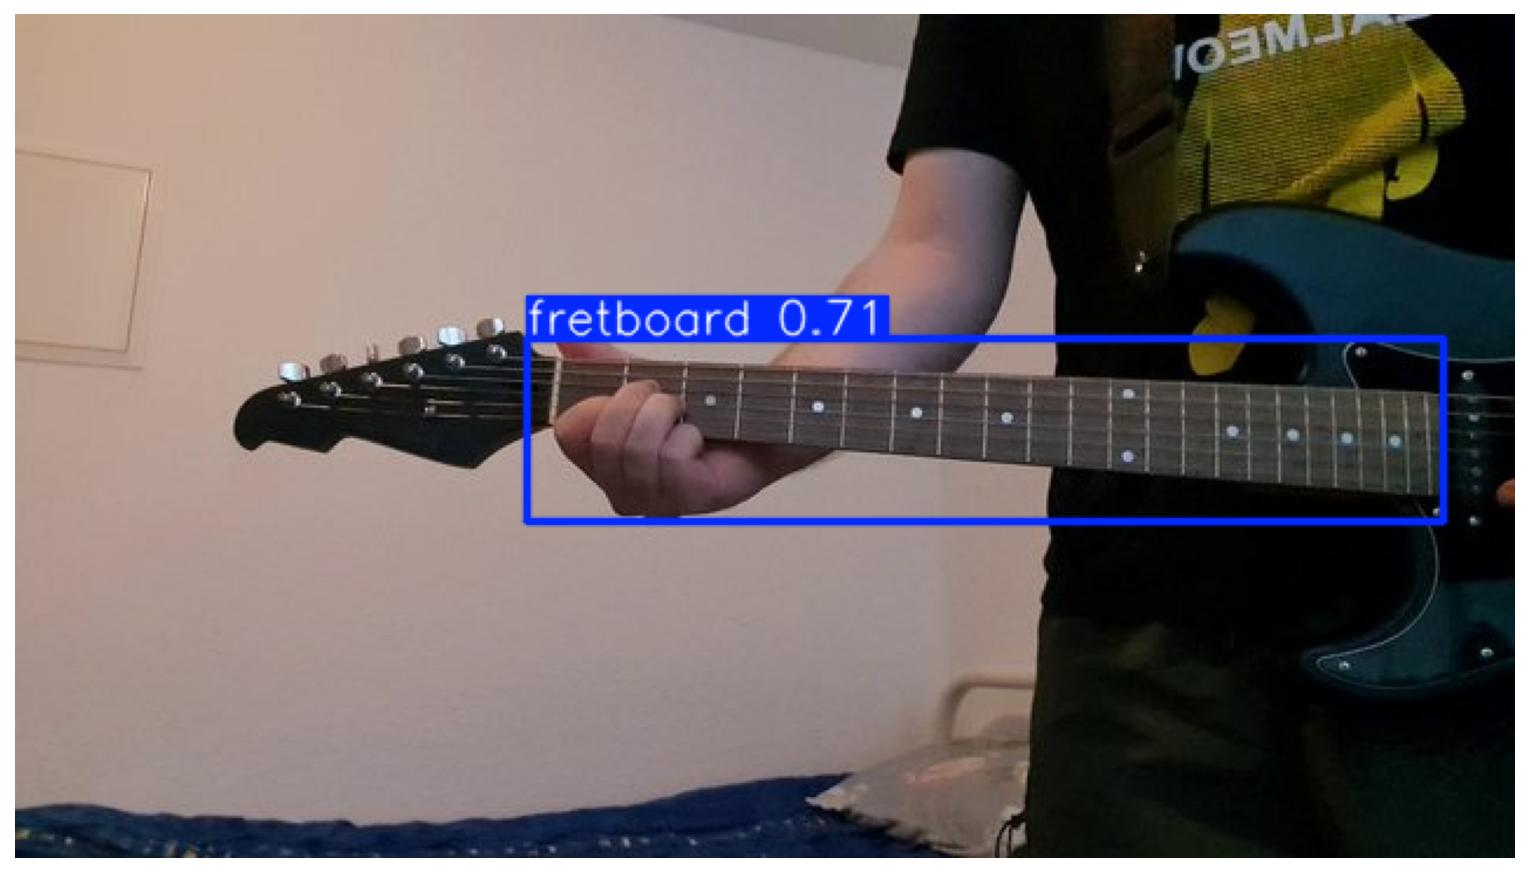
\includegraphics[width=\textwidth]{images/interim/dhimitrios-non-frozen.jpg}
    \end{minipage}
    \hfill
    \begin{minipage}{0.45\textwidth}
        \centering
        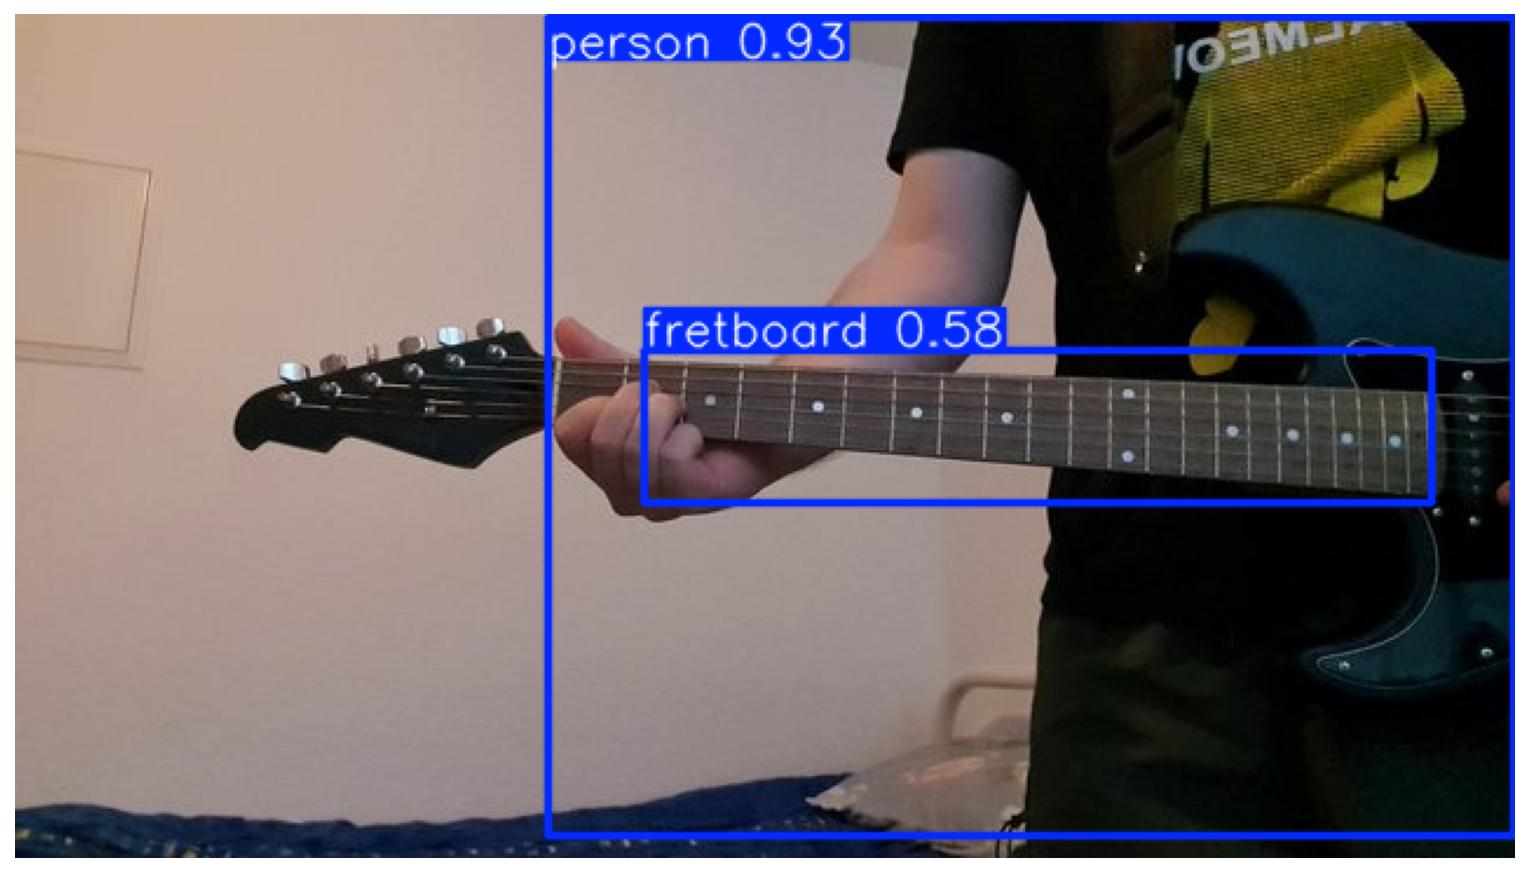
\includegraphics[width=\textwidth]{images/interim/dhimitrios.jpg}
    \end{minipage}
    \caption{\textbf{Left:} Prediction of our YOLOv9 \emph{fretboard detection model} finetuned without freezing the backbone. \textbf{Right:} Prediction of our YOLOv9 \emph{fretboard detection model} finetuned freezing every layer except the last one.}
    \label{fig:dataset-example}
\end{figure*}

\begin{figure*}[h]
    \begin{minipage}{0.33\textwidth}
        \centering
        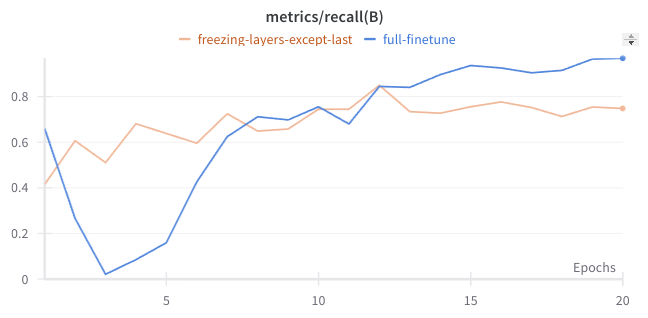
\includegraphics[width=\textwidth]{images/interim/metrics-recall-fretboard.png}
    \end{minipage}
    \hfill
    \begin{minipage}{0.33\textwidth}
        \centering
        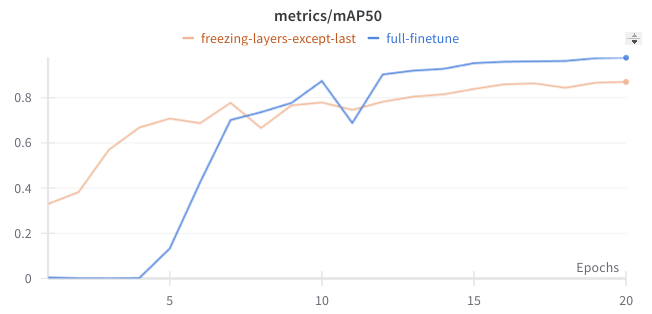
\includegraphics[width=\textwidth]{images/interim/metrics-mAP50-fretboard.png}
    \end{minipage}
    \hfill
    \begin{minipage}{0.33\textwidth}
        \centering
        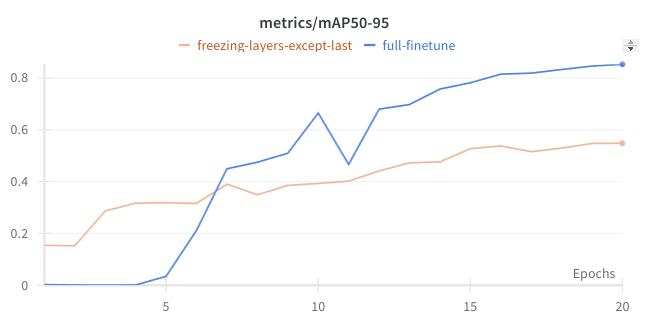
\includegraphics[width=\textwidth]{images/interim/metrics-mAP50-95-fretboard.png}
    \end{minipage}
    \caption{Plots for the two methods used to finetune our \emph{fretboard detection model}. \textbf{Left:} Recall. \textbf{Center:} mAP50. \textbf{Right:} mAP50-95.} 
    \label{fig:metrics-fretboard}
\end{figure*}

\section{Fretboard Detection}
For our \emph{fretboard detection model}, we used a YOLOv9 backbone \cite{wang2024yolov9} pretrained on the COCO dataset. We tried two different fine-tuning methods: freezing every layer except the last one and not freezing any layer, that is, finetuning the whole model. The results of the two methods are shown in \cref{fig:dataset-example} and in \cref{fig:metrics-fretboard}. 

Both methods are fundamentally different and serve different purposes. The first method is used to finetune the model to a specific task while keeping the backbone as it is. This allows us to keep the previous learned features and classes, i.e, the original 80 classes of the COCO dataset \cite{lin2015microsoftcococommonobjects}. On the other hand, the second method will finetune the whole model to the new task, while forgetting the previous learned features and classes. That is, the latter will have 2 classes after finetuning, the fretboard and the background.

Table \ref{tab:fretboard-metrics} shows the metrics for the two methods. The results show that the full finetuning achieve the best metrics, with a precision of 96.4\%, a recall of 96.81\%, a mAP50 of 97.8\%, and a mAP50-95 of 85.3\%. On the other hand, the model finetuned by freezing every layer except the last one has a precision of 82.42\%, a recall of 74.80\%, a mAP50 of 87.02\%, and a mAP50-95 of 54.78\%. Eventhough the full finetuning method achieved better metrics, the other method has the added benefit that it will still predict the other 80 classes of the COCO dataset, plus the new \emph{fretboard} class. See \cref{fig:dataset-example} for a visual comparison of the two methods, where the left image shows only the \emph{fretboard} class and the right image shows the \emph{fretboard} class plus the other detected classes of the COCO dataset.

\begin{table}[h!]
    \centering
    \caption{Summary of metrics for the 2 methods used to finetune our \emph{fretboard detection model}.}
    \begin{tabular}{lcc}
        \toprule
        \textbf{Metric} & \textbf{Freezing layers except last} & \textbf{Full finetune} \\
        \midrule
        Precision (B)   & 0.8242 & 0.9643 \\
        Recall (B)      & 0.7480 & 0.9681 \\
        mAP50           & 0.8702 & 0.9778 \\
        mAP50-95        & 0.5478 & 0.8530 \\
        \bottomrule
    \end{tabular}
    \label{tab:fretboard-metrics}
\end{table}

\section{Fine Tuning Visual Transformer (ViT)}
Different fine tuning methods were tried to adapt ViT to our inputs.
\subsection{Full Fine Tuning}
We first tried to fine tune the whole model. This was done by specifying the labels of our inputs to the pretrained model and it will attach a new MLP head to the classifier of the model which fits the dimensions of our labels and then the whole model were trained. We are getting a decent accuracy after adapting the model. \textbf{Attach figure of full fine tuning accuracy here.}
\subsection{Fine-tuning ViT for chord classification}
We tried to fine-tune the Vision Transformer (ViT) model for chord classification using different approaches.

\subsubsection{Training only the MLP head}
We first tried fine-tuning only the MLP head of ViT. This was done by freezing the weights of the model and only training the weights and biases of the classifier. We suspect that the pre-trained model is not able to capture the features of our inputs and the extended MLP head is merely trying to predict the labels on its own i.e. the same as a feed-forward network, thus achieving a very low accuracy of 18.2\% in the validation set of the enriched dataset. We also tried to unfreeze more layers of the model and they also didn't meet the expectation but the accuracy did increase which sort of confirms our suspicion.

\subsubsection{Full Fine Tuning}
In our next approach, we implemented full fine-tuning of the entire model. This process involved specifying the labels of our inputs to the pre-trained model, which then automatically attached a new Multi-Layer Perceptron (MLP) head to its classifier. The results of this method were encouraging, as we observed a good performance on our task. Most notably, we achieved an accuracy of 86\% on the validation set of the enriched dataset.

\subsubsection{Using PEFT methods}
As our next step, we are also planning to use PEFT \cite{peft} method to fine-tune the model. Specifically, we plan to use LoRA to reduce the number of parameters. We are still in the process of trying this method and we are expecting to see some improvements in training time without compromising on accuracy.

\section{Problems Encountered}
We encountered several issues during our work. Firstly, we faced some problems with the cluster. At first, we could not configure a conda environment or run our code. After some debugging, we were able to solve the problem by installing the packages in chunks instead of all at once.

Second, we faced some problems while fine-tuning YOLOv9 for fretboard detection. At first, we were using Ultralytics to fine-tune the model. However, we noticed that the final model recognized only two classes: the fretboard and the background. This meant that the model was forgetting all other classes on which it was trained. We addressed this problem by implementing another approach based on \cite{Extendin94:online}.

Lastly, during the classification phase, we faced some problems with data leakage. We noticed a rather high classification accuracy of 99\% in the validation set which was surprising to us. After some debugging, we found out that the problem originated from the preprocessing that we had applied to our classification dataset.


    %%%%%%%%% REFERENCES
    {\small
        \bibliographystyle{ieee_fullname}
        \bibliography{references}
    }

\end{document}
